\documentclass[fleqn]{article}
\usepackage[utf8]{inputenc}
\usepackage[margin=2cm]{geometry}

\usepackage{graphicx}
\usepackage{tikz}
\usepackage{enumitem}

% custom header/footer
\usepackage{fancyhdr}
\pagestyle{fancy}
\renewcommand{\headrulewidth}{0pt}
\fancyhf{}
\rfoot{\textsf{\thepage}}
\lfoot{\textsf{Suzie Brown}}

%annotations
\usepackage{color}
\usepackage{xspace}
\newcommand{\seb}[1]{\xspace\textcolor{red}{#1}\xspace}

%bibliography
\usepackage[style=authoryear, citestyle=authoryear-comp, sorting=nyt, backend=biber]{biblatex}
\addbibresource{../smc.bib}

% maths
\usepackage{amsmath}
\usepackage{amssymb}
\usepackage{amsthm}
\newtheorem{theorem}{Theorem}
\newtheorem{lemma}{Lemma}
\newcommand{\Prob}{\mathbb{P}}
\newcommand{\E}{\mathbb{E}}
\newcommand{\Et}{\mathbb{E}_t}
\newcommand{\V}{\operatorname{Var}}
\newcommand{\I}[1]{\mathbb{I}_{\{#1\}}}
\newcommand{\1}[1]{\mathbb{I}_{#1}}
\newcommand{\Mn}{\operatorname{Multinomial}}
\newcommand{\Bern}{\operatorname{Bernoulli}}
\newcommand{\Bin}{\operatorname{Binomial}}
\newcommand{\flnw}[1][i]{\lfloor N w_t^{(#1)} \rfloor}

\title{Bits of maths that didn't make it into the thesis}
\author{Suzie Brown}
\date{12 August 2021}

\begin{document}
\maketitle
\thispagestyle{fancy}


\section{Resampling parental indices or offspring counts?}
Another ``property'' of resampling schemes. Does it directly sample the parental indices (and then offspring counts can be calculated), or does it directly sample offspring counts (and parental indices can then be assigned e.g.\ uniformly under these counts)?

\vspace*{7pt}
\begin{tabular}{l l}
Resampling scheme & Directly samples \\
\hline
\texttt{multi} & parental indices \\
\texttt{star} & parental indices \\
\texttt{strat} & parental indices \\
\texttt{strat-roulette} & parental indices \\
\texttt{syst} & parental indices \\
\texttt{res-multi} & offspring counts \\
\texttt{res-star} & offspring counts \\
\texttt{res-strat} & offspring counts \\
\texttt{res-syst} & offspring counts \\
\texttt{ssp} & offspring counts \\
\texttt{mvb} & offspring counts \\
\end{tabular}
\vspace*{7pt}

Schemes based on inversion sampling (even roulette-style) transform each input point $u_i$ into a parental index. 
Under star resampling, the parental indices and offspring counts contain the same information, so it can be equivalently formulated either way, but I've defined it as sampling one parent and then assigning all the offspring to that parent.
The determinstic part of residual schemes does not specify particular parents, even if the stochastic part might.
The SSP scheme is presented in terms of an algorithm for calculating offspring counts. 
The MVB scheme doesn't specify a particular algorithm but is defined in terms of the distribution of offspring counts, not parental indices.


\section{Probability of killing a low-weight particle}
This is another property of resampling schemes which I didn't include in the thesis. However it is very tractable and it leads to an alternative partial ordering (cf. thesis Figure 2.9) with a reasonable interpretation.

Suppose $w_t^{(i)} = \delta/N$ where $\delta \in [0,1)$.
What is the probability that $\nu_t^{(i)} =0$ under each resampling scheme?

\subsection*{Multinomial}
\begin{equation*}
\Prob[ \nu_t^{(i)} =0 \mid w_t ]
= \Prob[ \Bin(N, \delta/N) =0 ]
= \left( 1- \frac{\delta}{N} \right)^N .
\end{equation*}

\subsection*{Residual-multinomial}
Deterministic part is zero.
\begin{equation*}
\Prob[ \nu_t^{(i)} =0 \mid w_t ]
= \Prob[ \Bin(R, r_i) =0 ]
= \left( 1- r_i \right)^R 
= \left( 1- \frac{\delta}{R} \right)^R .
\end{equation*}

\subsection*{Star}
\begin{equation*}
\Prob[ \nu_t^{(i)} =0 \mid w_t ]
= \Prob[ \Bern(\delta/N) =0 ]
= 1- \frac{\delta}{N} .
\end{equation*}

\subsection*{Residual-star}
Deterministic part is zero.
\begin{equation*}
\Prob[ \nu_t^{(i)} =0 \mid w_t ]
= \Prob[ \Bern(r_i) =0 ]
= 1- r_i
= 1- \frac{\delta}{R} .
\end{equation*}

\subsection*{Stratified}
Using Table 2.2 in thesis, with $\delta_L \in [0,\delta]$,
\begin{equation*}
\Prob[ \nu_t^{(i)} =0 \mid w_t ]
= 1 - \delta + \delta_L (\delta - \delta_L)
\in \left[ 1-\delta, 1- \frac{3}{4}\delta \right] .
\end{equation*}

\subsection*{Residual-stratified}
Same as stratified, since there is no deterministic part:
\begin{equation*}
\Prob[ \nu_t^{(i)} =0 \mid w_t ]
= 1 - \delta + \delta_L (\delta - \delta_L)
\in \left[ 1-\delta, 1- \frac{3}{4}\delta \right] .
\end{equation*}

\subsection*{Stochastic rounding}
\begin{equation*}
\Prob[ \nu_t^{(i)} =0 \mid w_t ]
= \Prob[ \nu_t^{(i)} = \flnw \mid w_t ]
= 1 - \delta .
\end{equation*}

\subsection{Interpretation}
The above quantities admit some inequalities, implying a partial ordering among resampling schemes. These inequalities are represented in the following graph, where $\Prob[ \nu_t^{(i)} =0 \mid w_t ]$ is non-increasing along arrows. The dashed arrow indicates an inequality that holds iff $R>1$ (if $R=1$ the inequality goes the other way). The quantity under consideration is equal for straitfied and residual-stratified resampling. The missing arrows (those which are not implied by paths of arrows) represent quantities which do not admit an inequality holding for all $\delta, N$.\\

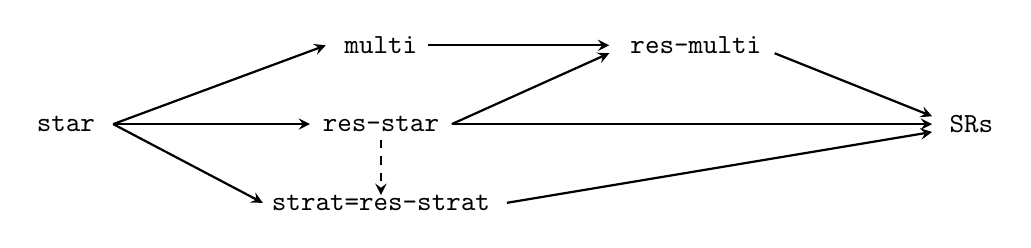
\begin{tikzpicture}[>=stealth]
\node at (0,0) {\texttt{star}};
\node at (4,1) {\texttt{multi}};
\node at (4,0) {\texttt{res-star}};
\node at (4,-1) {\texttt{strat=res-strat}};
\node at (8,1) {\texttt{res-multi}};
\node at (11.5,0) {\texttt{SRs}};
\draw[->, thick] (0.6,0)--(3.3,1); %% star -> multi
\draw[->, thick] (0.6,0)--(3.1,0); %% star -> res-star
\draw[->, thick] (4.6,1)--(6.9,1); %% multi -> res-multi
\draw[->, thick] (4.9,0)--(6.9,0.9); %% res-star -> res-multi
\draw[->, thick] (5.6,-1)--(11,-0.1); %% strat -> SR
\draw[->, thick] (9,0.9)--(11,0.1); %% res-multi -> SR
\draw[->, thick] (4.9,0)--(11,0); %% res-star -> SR
\draw[->, thick] (0.6,0)--(2.5,-1); %% star -> strat
\draw[->, thick, dashed] (4,-0.2)--(4,-0.9); %% res-star -> strat
\end{tikzpicture}

\vspace*{5pt}
Since $\E[ \nu_t^{(i)} \mid w_t ]$ is equal across all resampling schemes (ensured by the unbiasedness property), the probability under consideration is capturing the spread around this mean value. Larger values of $\Prob[ \nu_t^{(i)} =0 \mid w_t ]$ must be compensating for higher mass on large values of $\nu_t^{(i)}$ (in the sense of its conditional PMF).
It is not surprising then that SRs come out smaller than everything else (since they give the lowest possible conditional variance of $\nu_t^{(i)}$, with mass only on 0 and 1) and that star resampling comes out bigger than everything else (since it gives the highest possible conditional variance of $\nu_t^{(i)}$, with mass only on 0 and $N$).



\section{Properties of stratified roulette resampling}
I have noted that Whitley's ``roulette wheel'' is an equivalent definition to the usual inversion sampling one in the case of systematic (or multinomial) resampling, but that these representations are not equivalent for stratified resampling. Indeed, the roulette wheel version is always ``worse'' because it unnecessarily adds extra randomness. In fairness, Whitley never proposed to use the roulette wheel for stratified resampling.

I didn't include the roulette version of stratified resampling in the analysis of resampling schemes, but I initially did some of the calculations as if I were going to include it. Here are those.


\subsection*{Degenerate under equal weights?}
Standard stratified resampling: YES\\
Roulette stratified resampling: NO\\[5pt]
When all weights are multiples of $1/N$, the sampling intervals still do not generally line up with the weight intervals (whereas they do in standard stratified resampling). It is therefore possible for the offspring counts to deviate from their means by $1$ in either direction.


\subsection*{Marginal support of offspring counts}
Standard stratified resampling: $\{K-1, K, K+1, K+2\}$\\
Roulette stratified resampling: $\{K-1, K, K+1, K+2\}$\\
(given $w_t^{(i)} = \frac{K+\delta}{N}$)\\[5pt]
This follows from the same reasoning as usual (just draw a picture).


\subsection*{Marginal variance of offspring counts}
Standard stratified resampling: $\leq 2$\\
Roulette stratified resampling: $\leq 2$\\[5pt]
I haven't got the calculations here, but according to my notes the best upper bound I could find was the same in each case. This doesn't mean the actual variance is the same for both, just the bounds on the variance. I haven't attempted a direct comparison for say the same vector of weights under both resampling schemes, but I imagine there are some complications with doing such a calculation.


\subsection*{Monte Carlo variance}
I would expect that perhaps the roulette version has higher variance, because of the additional randomness involved. I haven't proved it though.


\subsection*{Exchangeability}
Standard stratified resampling: NO\\
Roulette stratified resampling: NO\\[5pt]
It is not as obvious with the roulette wheel, because for instance offspring 1 is no more likely to choose parent 1 than offspring N is. But if you look at the joint distribution of parental indices you can see that it does not leave the offspring exchangeable. For instance, consecutive offspring tend to have parents that are near to each other, while two offspring with distant indices do not.


\subsection*{Permutation sensitivity}
Standard stratified resampling: YES\\
Roulette stratified resampling: ?\\[5pt]
I think probably yes, but I haven't proved it.


\subsection*{Computational complexity}
Standard stratified resampling: $O(N)$\\
Roulette stratified resampling: $O(N)$\\[5pt]
Adding a phase to each $u_i$ requires at most $O(N)$ operations. I suspect that in practice the two algorithms in fact differ by only a constant number of operations.


\subsection*{Negative association}
Standard stratified resampling: YES\\
Roulette stratified resampling: ?


\subsection*{Star discrepancy}
Standard stratified resampling: $\in [1/(2N), 1/N]$\\
Roulette stratified resampling: $\in [1/(2N), 2/N]$\\[5pt]
The best case is the same: in theory both standard and roulette versions can attain the regular grid with discrepancy $1/(2N)$.
But the worst case for roulette version is much worse than the standard case, because it is possible for example for two points to fall arbitrarily close to zero. 
This is really just a feature of the definition of star discrepancy, which is more compatible with the standard inversion sampling than with the roulette wheel; one could define a star discrepancy on the wheel and then we would see no difference between the two formulations of stratified resampling.


\subsection*{Conditional independence}
Standard stratified resampling: YES\\
Roulette stratified resampling: ?\\[5pt]
Do you lose conditional independence because all sampled points share a common phase? Or are the points still independent because we can treat the phase as part of the original distribution of sampled points?









\printbibliography
\end{document}